\documentclass[a4paper, norsk, 9.8pt]{article} % Define document type and size
%% LaTeX Preamble - Common packages

\usepackage{array, xcolor} % Table packages
\usepackage{url} %Package for formating url properly use \url{www.example.com}


%% Three packages for handling norwegian symbols
\usepackage[utf8]{inputenc}
\usepackage[norsk]{babel}
\usepackage[T1]{fontenc}
\usepackage{marvosym}
\usepackage{hyperref}
\hypersetup{
    colorlinks = true,
    linkbordercolor = {white},
    allcolors = cyan
}

\usepackage{graphicx} % Package for handling figures and pictures
\usepackage{caption}
\usepackage{subcaption} % Package for handling captions
\usepackage{calc} % LaTeX calculates for instance width from algebraic expressions
\usepackage{enumitem} % List woth numbers
\usepackage{longtable}

\setlength{\voffset}{-45pt}
\setlength{\textheight}{730pt}
\setlength{\topmargin}{-5pt}
\setlength{\headsep}{0pt}
\setlength{\textwidth}{500pt}
\setlength{\hoffset}{-70pt}
%\usepackage{color}

%%%%
%% DEFINE TABLE SETTINGS
%%%%
\definecolor{lightgray}{gray}{0.8}
\newcolumntype{L}{>
{\raggedleft}p{0.16\textwidth}} % 0.14
\newcolumntype{R}{p{0.84\textwidth - 4\tabcolsep}} % subtract off 4 times \tabcolsep

\newcommand\VRule{\color{cyan}\vrule width 1pt}

\title{}
\author{}
\date{}


\begin{document}
\pagenumbering{gobble} % Remove pagenumbering

%%%%
%% INSERT PICTURE
%%%%
\begin{figure}[h]
\begin{subfigure}[b]{2.7cm}
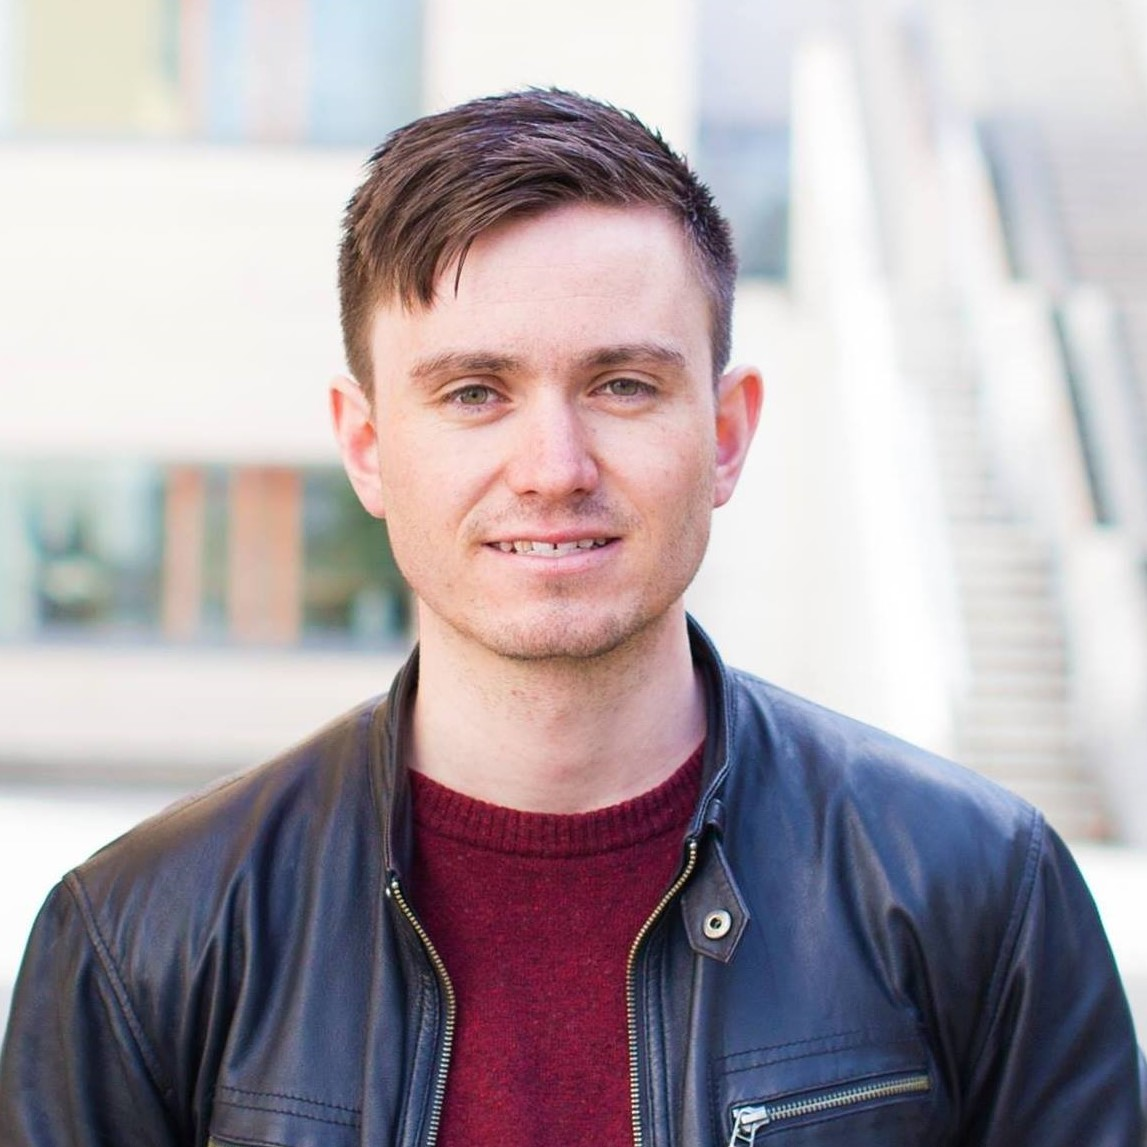
\includegraphics[scale = 0.064]{bilde_1.jpg}
\end{subfigure}
\begin{subfigure}[b]{9cm}
   	\textsc{\bfseries{\Huge{Thomas Kleiven}}} \\[5pt]
   	\textsc{\Large{Engineering and ICT}} \\[5pt]
   	\textsc{\Large{Curriculum Vitae}}
\end{subfigure}
\end{figure}

%%%%
%% INSERT ADDRESS AND CONTACT INFORMATION
%%%%
\begin{table}[h]
\noindent \begin{tabular*}{\textwidth}{@{\extracolsep{\fill}} l r}
Edgar B. Schieldropsvei 100B & 19. June 1994 \\
7033 Trondheim & 
\includegraphics[scale=0.042]{phone.png}  +47 930 47 147\\
Norge
 & 
\includegraphics[scale=0.013]{mail.png} \href{mailto:thomas@isvik.no}{{thomas@isvik.no}} \\
 & 
\includegraphics[scale=0.020, trim={2mm 28mm 2mm 2mm}, clip]{linkedin_logo.png} \href{https://no.linkedin.com/in/thomaskleiven}{{thomaskleiven}} \\
 & 
\includegraphics[scale=0.013, trim={0mm 0mm 75mm 0mm}, clip]{github.png} \href{https://github.com/thomaskleiven}{{thomaskleiven}}
\end{tabular*}
\end{table}

\section*{Education}
\begin{tabular}{L!{\VRule}R}
2014 - & {\bf Master of Science, Engineering and ICT, Norwegian University of Science and Technology, Gløshaugen, Trondheim} \\
  & {Specialisation in Product Development and Process Engineering. This line of study focus on the demand for engineers with both ICT expertise and an advanced engineering education}
  \\
  \smallskip 2013 - 2014 & {\bf \smallskip Military service with His Majesty the King`s Guard} \\
    & {His Majesty the King's Guard Drill Team of Norway} \\
    \smallskip 2010-2013 & {\bf \smallskip Skeisvang vgs, Haugesund}  \\
\end{tabular}

\section*{Work Experience}
\begin{tabular}{L!{\VRule}R} 2016 & {\bf Statoil ASA - Summer Intern}
\\
& {Implemented an application in Java using JavaFX for GUI in addition to assisting \newline operators at the facility}
\\
\smallskip 2013 - 2016 & {\bf \smallskip Møbelringen Math. Lande AS} \\
& {Temporary employment - Storage Worker} \\
\smallskip 2008 - 2013 & {\bf \smallskip Maintainer at Isvik Helse AS}  \\
& {Temporary employment - Performed preventative and predictive maintenance on buildings and facilities}
\end{tabular}


\section*{Computer skills}
\begin{tabular}{L!{\VRule}R}
 OS & Windows, Macintosh , Linux\\
Programming & MATLAB, Java, C++, Python\\
Word processing & MS Office, \LaTeX \\
PLM Software & Siemens NX \\
ERP Systems & SAP, Microsoft Dynamics AX \\
Version Control & Git
\end{tabular}

\section*{Voluntary work}
\begin{tabular}{L!{\VRule}R}
2015 - 2017 & {\bf Chairman of the Board, NTNUI Triatlon} \\
& In charge of the daily administrative matters, in addition to planning the first Norwegian Student Championship in triathlon. During these last two years the number of members has more than doubled itself and we are now more than 70 members.
\end{tabular}

\section*{Languages}
\begin{tabular}{L!{\VRule}R}
Norwegian & Native speaker \\
English &  Fluent written and orally \\
German & Basic written and orally\\
\end{tabular}


%\section*{Vedlegg}





\end{document}
